% L13c figure: the architecture of the Model Context Protocol (MCP).
%
% A user talks to a host. Inside the host, a language model and one client for
% each server. Each client exchanges MCP messages with one server. Each server
% calls a web API over HTTPS: the weather server calls the NWS API, and the
% FRED server calls the FRED API.
%
% Drawn on November 12, 2026 with the palette and build of the L13a figures.
% The notebook SVG carries a dark palette added by theme_svg.py; keep new
% colors in that script's mapping when changing the palette here.
\documentclass[tikz,border=4pt]{standalone}
\usepackage[no-math]{fontspec}
\IfFontExistsTF{Arial}{\setsansfont{Arial}}{\setsansfont{TeX Gyre Heros}}
\renewcommand{\familydefault}{\sfdefault}
\usepackage{amsmath,amssymb}
\usetikzlibrary{arrows.meta, calc, fit, backgrounds}

% Ink, blue, gray, and band match the L13a figures. Blue marks the MCP messages.
\definecolor{vnink}{HTML}{202124}
\definecolor{gdblue}{HTML}{0091FF}
\definecolor{gdgray}{HTML}{6D7278}
\definecolor{waband}{HTML}{EEF0F2}
\definecolor{nodefill}{HTML}{FFFFFF}

\begin{document}
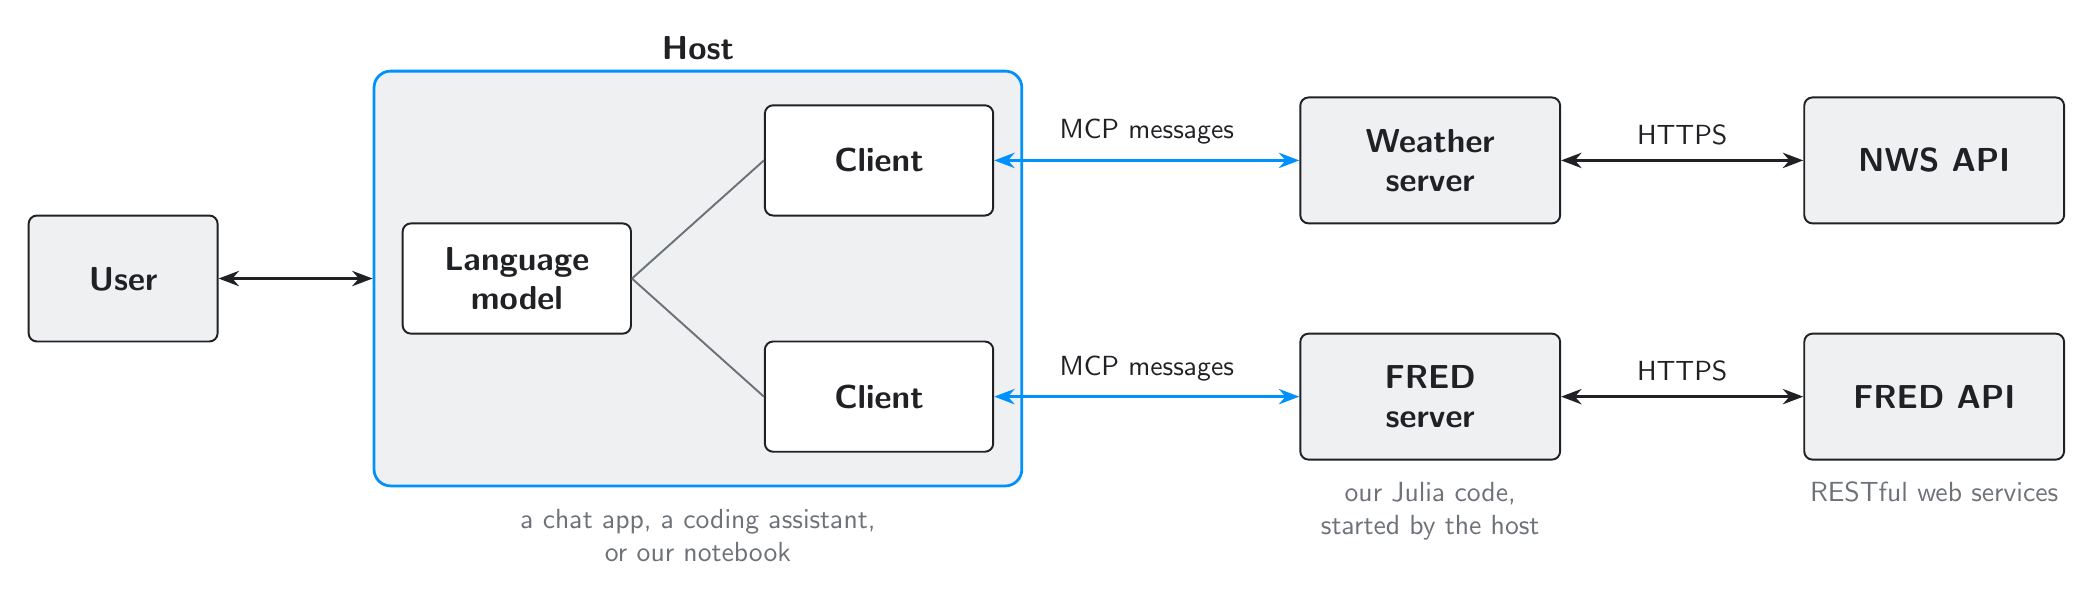
\begin{tikzpicture}[
  font=\sffamily\large,
  >={Stealth[length=2.6mm]},
  box/.style={draw=vnink, rounded corners=3pt, minimum width=3.3cm, minimum height=1.6cm,
    fill=waband, line width=0.7pt, text=vnink, align=center, font=\sffamily\large\bfseries},
  inner/.style={draw=vnink, rounded corners=3pt, minimum width=2.9cm, minimum height=1.4cm,
    fill=nodefill, line width=0.7pt, text=vnink, align=center, font=\sffamily\large\bfseries},
  note/.style={font=\sffamily\normalsize, text=gdgray, align=center},
  msg/.style={font=\sffamily\normalsize, text=vnink, align=center},
  mcp/.style={<->, line width=1.0pt, draw=gdblue},
  https/.style={<->, line width=1.0pt, draw=vnink},
  local/.style={line width=0.7pt, draw=gdgray}
]

% ------------------------------------------------------------ the host
\node[inner] (model)  at (0.0, 0.0)  {Language\\model};
\node[inner] (client1) at (4.6, 1.5)  {Client};
\node[inner] (client2) at (4.6, -1.5) {Client};
\draw[local] (model.east) -- (client1.west);
\draw[local] (model.east) -- (client2.west);
\begin{scope}[on background layer]
  \node[draw=gdblue, rounded corners=6pt, line width=1.0pt, fill=waband,
    fit=(model)(client1)(client2), inner xsep=10pt, inner ysep=12pt] (host) {};
\end{scope}
\node[font=\sffamily\large\bfseries, text=vnink, anchor=south] at (host.north) {Host};
\node[note, anchor=north] at ($(host.south)+(0,-0.15)$) {a chat app, a coding assistant,\\or our notebook};

% ------------------------------------------------------------ the user
\node[box, minimum width=2.4cm] (user) at (-5.0, 0.0) {User};
\draw[https] (user.east) -- (host.west);

% ------------------------------------------------------------ the servers
\node[box] (server1) at (11.6, 1.5)  {Weather\\server};
\node[box] (server2) at (11.6, -1.5) {FRED\\server};
\draw[mcp] (client1.east) -- (server1.west) node[msg, midway, above=2pt] {MCP messages};
\draw[mcp] (client2.east) -- (server2.west) node[msg, midway, above=2pt] {MCP messages};
\node[note, anchor=north] at ($(server2.south)+(0,-0.15)$) {our Julia code,\\started by the host};

% ------------------------------------------------------------ the web APIs
\node[box] (api1) at (18.0, 1.5)  {NWS API};
\node[box] (api2) at (18.0, -1.5) {FRED API};
\draw[https] (server1.east) -- (api1.west) node[msg, midway, above=2pt] {HTTPS};
\draw[https] (server2.east) -- (api2.west) node[msg, midway, above=2pt] {HTTPS};
\node[note, anchor=north] at ($(api2.south)+(0,-0.15)$) {RESTful web services};

\end{tikzpicture}
\end{document}
